% Proste diagramy w tikz
% Galeria: https://tikz.net/
\documentclass{article}

\usepackage{tikz}
\usetikzlibrary{arrows.meta, positioning}

\begin{document}

	
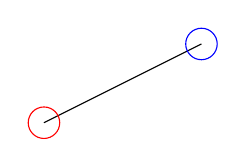
\begin{tikzpicture}
	\draw (0,0) -- (2,1);
	\draw[red] (0,0) circle (0.2);
	\draw[blue] (2,1) circle (0.2);
\end{tikzpicture}


\begin{tikzpicture}
	\node (A) at (0,0) {A};
	\node (B) at (2,1) {B};
	\draw[->] (A) -- (B);
\end{tikzpicture}



\begin{tikzpicture}[>=Stealth, node distance=2.5cm, auto]
	\node (X) {$X$};
	\node (Y) [right=of X] {$Y$};
	\node (Z) [right=of Y] {$Z$};

	\draw[->] (X) -- node[above] {$g$} (Y);
	\draw[->] (Y) -- node[above] {$f$} (Z);
	\draw[->, dashed, bend right=45] (X.south east) to node[below] {$f \circ g$} (Z.south west);
	
\end{tikzpicture}

% Bonus:
% "Generate a TikZ diagram showing a generic Venn diagram with semi-transparent red, green, and blue circles and thick outlines."
% GPT (nienajgorszy efekt, ale do poprawek):

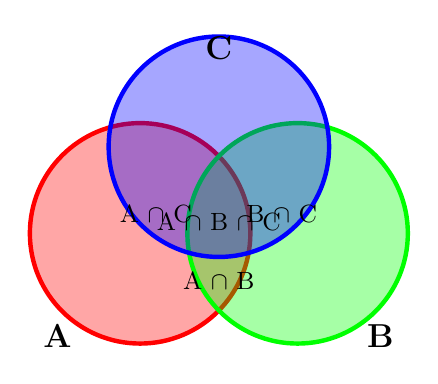
\begin{tikzpicture}[scale=1]
	
	% parameters
	\def\r{1.4}           % radius
	\def\oline{1.6pt}     % outline thickness
	
	% red circle (left)
	\fill[red, fill opacity=0.35] (-1,0) circle (\r);
	\draw[line width=\oline, red] (-1,0) circle (\r);
	
	% green circle (right)
	\fill[green, fill opacity=0.35] (1,0) circle (\r);
	\draw[line width=\oline, green] (1,0) circle (\r);
	
	% blue circle (top)
	\fill[blue, fill opacity=0.35] (0,1.1) circle (\r);
	\draw[line width=\oline, blue] (0,1.1) circle (\r);
	
	% optional set labels
	\node at (-2.05,-1.3) {\large \textbf{A}};
	\node at (2.05,-1.3)  {\large \textbf{B}};
	\node at (0,2.35)     {\large \textbf{C}};
	
	% example intersection labels (optional)
	\node[font=\small] at ( -0.8, 0.25) {A $\cap$ C};
	\node[font=\small] at (  0.8, 0.25) {B $\cap$ C};
	\node[font=\small] at (  0.0,-0.6) {A $\cap$ B};
	\node[font=\small] at (  0.0, 0.15) {A $\cap$ B $\cap$ C};
	
\end{tikzpicture}

\end{document}
